

\section{State of the art and objectives}

Heat flows from warmer to cooler bodies until thermal equilibrium is reached, according to the second law of thermodynamics. Contrasting heat transfer is crucial for energy-conservation purposes, while leveraging it is instrumental in many energy-conversion technologies. Several other otherwise unrelated technologies rely on accurate \emph{heat management}, \emph{i.e.} on our capacity to maintain the temperature of a device within a prescribed operating range, which depends in turn on the relative strength of heat production, by Joule or other dissipative mechanisms, and outflux.\cite{Cahill2003,Pop:2010dv,Cahill:2014bx,Shi:2015io,Volz:2016ky} Heat flow determines the cooling/heating rates and internal temperature distribution of out-of-equilibrium systems: for this reason, fathoming it is crucial for understanding the thermal history of the Earth and other planets, one of our main sources of knowledge about their origin, evolution, and present state of their interiors,\cite{Hubbard:1984} with such important implications as volcanology and seismology.\cite{Duarte2016}

Heat transfer occurs via three distinct mechanisms that may prevail or coexist in different regimes:\cite{Lienhard2017} in \emph{convection}, heat is transported by a flowing mass; in \emph{radiation} it is removed from the surface of the hot source by photons, while in \emph{conduction} heat transfer is determined by the microscopic dynamics of the atoms or, in the case of metals, of conduction electrons.\cite{ziman,Tritt2004} Radiation is mostly a surface phenomenon: it plays a role at room temperature in nanodevices as ``near-field radiation'' across nanoscale gaps,\cite{Rousseau:2009es} while in the bulk it becomes significant at high temperatures. Convection only occurs in liquids and, on geological time scales, in viscous solids.\cite{Schibert2001} In bulk solid-state technologies conduction is therefore the only relevant heat-transfer mechanism. In liquid-state technologies, instead, convection and conduction may coexist and the efficiency of thermal conduction often depends on the relative magnitude of the heat fluxes associated with the two mechanisms. At planetary conditions the three mechanisms may coexist.\cite{Hubbard:1984} Although convection is thought to prevail in most cases of physical interest, heat transfer across distinct homogeneously convecting layers is entirely determined by conduction. Hence, understanding heat conduction is crucial to unravel the mechanisms of heat transfer in all cases of scientific and technological interest. 

The past few decades have witnessed a staggering increase in our ability to understand the properties of matter by combining the laws of statistical physics and quantum mechanics with ever more sophisticated algorithms to implement them on computers of ever increasing power. In condensed-matter physics and materials science the scope of computer simulation has been vastly widened by density functional theory (DFT),\cite{Hohenberg1964,Kohn1965,MRS-DFT,Jain2016,Gillan2006} which allows describing inter-atomic forces entirely from first principles (``\emph{ab initio}''), using the chemical composition and the fundamental laws of nature as the sole ingredients, thus freeing molecular simulations from the need to leverage prior experimental knowledge of these interactions, which may be unavailable or not accurate enough.

The most important property characterizing heat transport in materials is the \emph{thermal conductivity}, $\kappa$, defined as the ratio between the magnitude of the heat flux, $\mathbf{J}$, and the temperature gradient:
\begin{linenomath}\begin{equation}
\mathbf{J}= -\kappa \nabla T. \label{eq:kappa}
\end{equation}\end{linenomath}
Notwithstanding its fundamental importance, \emph{thermal conductivity has proven to be one of the most difficult transport coefficients to calculate} [Ref. \citenum{Evans1990}, p.149] and its simulation is still today a conceptual, no less than practical, challenge to our materials modeling capabilities. Different approaches are available to model heat conduction in different materials and regimes. In THETIS we will address insulators, where heat transport is determined by the dissipative dynamics of atoms, the electrons following adiabatically in their ground state. We will refer to this regime as to atomic or \emph{adiabatic heat conduction}. Simulating adiabatic heat conduction usually relies on the Boltzmann's transport equation (BTE),\cite{Peierls1929,Zhou2016} on non-equilibrium Green's functions (NEGF), \cite{Wang2008} or on molecular dynamics (MD),\cite{Allen1989,Frenkel2001} both in its non-equilibrium and equilibrium flavors. NEGF's are designed to compute the conductance of open systems, such as nanoscale devices and interfaces, but they do not apply to bulk conduction, which is the main focus of THETIS. The BTE is the method of choice for crystals well below melting, where long-lived phonons are clearly identified as the heat carriers. In this case density-functional perturbation theory\cite{Baroni1987a,Gonze1989,Baroni2001} allows one to compute accurate phonon frequencies \cite{Giannozzi1991} and lifetimes,\cite{Debernardi1995,Paulatto2013} and thus implement the BTE entirely from first principles.\cite{Broido:2007iu} The flexibility and accuracy of \emph{ab initio} BTE are such that this approach is being successfully used to screen new materials for custom-designed properties, such as high thermal conductivity for passive cooling\cite{Lindsay:2013fw,Lindsay:2013db} or very thermal conductivity for thermoelectric energy conversion.\cite{PhysRevX.4.011019,Schwingen2014} Recent self-consistent and variational approaches to solve the BTE beyond the relaxation-time approximation \cite{Fugallo2013} are also providing fresh and deep insight into the collective character of heat transport.\cite{Fugallo2013,Lee:2015ex,Cepellotti2015,Cepellotti:2016bk} Yet, the applicability of \emph{ab initio} BTE is not only restricted to periodic systems consisting of a small number of atoms per unit cell (the computational cost scales in between the fourth and fifth power of this number according to the implementation, and convergence is often tricky), but it is severely limited by its own inherent approximations: as the temperature increases, anharmonic effects become so important as to eventually make it break down well below melting,\cite{Turney:2009bb} while the BTE simply does not apply to glasses and liquids, where phonons are not even defined.\cite{Allen1989} MD is set to overcome these limitations. In non-equilibrium MD (NEMD),\cite{Evans1990,Muller-Plathe1997} or in its ``approach-to-equilibrium'' (AEMD) variant,\cite{Lampin2013} temperature gradients or heat fluxes are explicitly imposed on the virtual sample, and the transport coefficients estimated from the value of the conjugate variable (flux or gradient) thus generated in NEMD, or from the time it takes for the sample to equilibrate in AEMD. NEMD and AEMD lend themselves to a straightforward  quantum-mechanical implementation \cite{Stackhouse2010b,Bouzid2017} using \emph{ab initio} molecular dynamics (AIMD),\cite{Car1985,Marx2009} but they may be both affected by non-linear effects, due to the strength of the temperature gradient to be imposed\cite{Schelling2002,He2012} and by finite-size/finite-time effects that require long simulation times and cumbersome extrapolations to the thermodynamic limit to be tamed.\cite{sellan2010,He2011,He2012,Zaoui2016,Wang2017} We believe that a full deployment of the predictive power of modern simulation methods to heat transport in liquids and in amorphous and strongly anharmonic crystalline solids can only build on a combination of equilibrium MD techniques, based on the Green-Kubo (GK) theory of linear response, with DFT, an endeavor that was deemed impossible until recently\cite{Marcolongo2016} and that we want to lead to successful completion in THETIS. This feat will pave the way to solve a number of outstanding problems in the science of planetary evolution and in the technology of energy materials, where disorder and anharmonicity play a fundamental role and the modeling approaches available to date are bound to fail.

\subsubsection*{Kohn and Sham finally meet Green and Kubo}
The rigorous theory of heat conduction in materials, based on the microscopic interactions and dynamics of their molecular constituents, is a cornerstone of modern condensed-matter physics and one of the early feats of non-equilibrium statistical mechanics.\cite{Kubo1991} This program, initiated by Onsager in the thirties\cite{Onsager1931a,Onsager1931b} and carried on by Green\cite{Green1952,Green1954} and Kubo\cite{Kubo1957a,Kubo1957b} in the fifties, posits on the adiabatic decoupling of the slow long-wavelength components of the densities of conserved extensive quantities (energy, momentum, and particle numbers),\cite{Kadanoff1963} the so-called \emph{hydrodynamic variables}, from the other atomically fast degrees of freedom. One of its most important results is the relation between the transport coefficients relating the intensity of a flux, $J$, with the magnitude of the conjugate force (such as the heat flux and temperature gradient in Eq. \ref{eq:kappa}) and the auto-correlation times of the flux: 
\begin{linenomath}\begin{equation}
\kappa\propto\int_{0}^{\infty}\!\langle{J}(t){J}(0)\rangle\, dt,\label{eq:GK}
\end{equation}\end{linenomath}
where the brackets indicate ensemble averages over trajectories. In equilibrium MD these ensemble averages can be evaluated in principle as lagged-product autocovariances of the heat-flux time series, and are thus readily available to numerical simulation. In the following the integral in Eq. \eqref{eq:GK} will be sometimes referred to as the \emph{GK integral}. In many ways the resulting approach to thermal transport, that we will dub as \emph{GKMD}, is the method of choice for strongly anharmonic and/or disordered systems (liquids, glasses, and crystalline solids at hight temperature and/or containing very mobile species), where the BTE does not apply and NEMD is subject to non-trivial practical limitations. 

\begin{figure}[t]
\hbox to \hsize{\hfill
\begin{minipage}{0.45\textwidth}
\centering 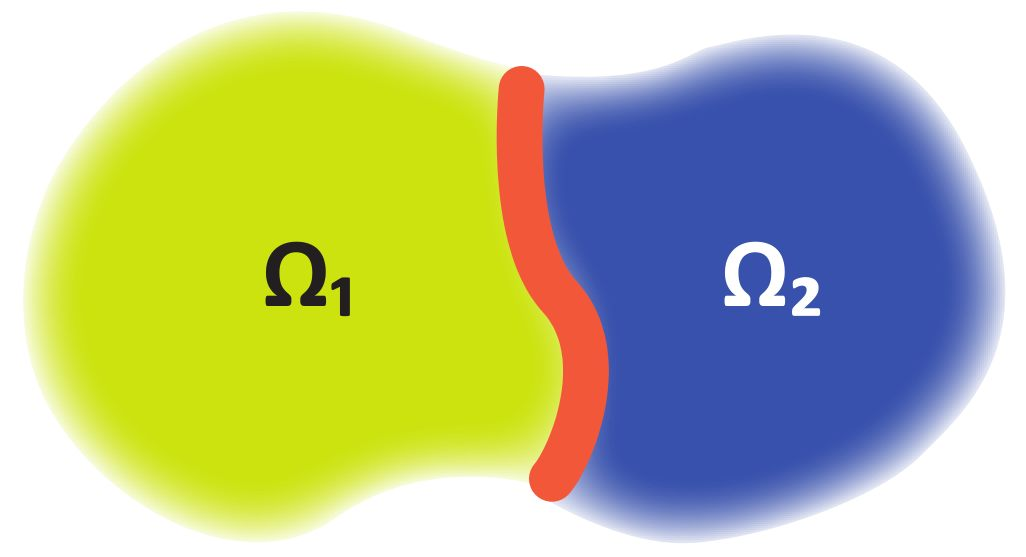
\includegraphics[width=0.8\textwidth]{blob}
\end{minipage}
\hfill
\begin{minipage}{0.45\textwidth}
\begin{align}
\phantom{E(\Omega_{1}\cup\Omega_2)}
&\begin{aligned}
  \mathllap{E(\Omega_{1}\cup\Omega_2)} &= E(\Omega_1) + E(\Omega_2) + W_{12}\\
    & \overset{?}{=}\mathcal{E}(\Omega_1)+\mathcal{E}(\Omega_2)
  \end{aligned} \nonumber \\[12pt]
&\begin{aligned}
  \mathllap{\mathcal{E}(\Omega_1)} &= E(\Omega_1) +\alpha W_{12} \\
  \mathllap{\mathcal{E}(\Omega_2)} &= E(\Omega_2) +(1-\alpha) W_{12}
\end{aligned}
\label{eq:extensivity}
\end{align}
\end{minipage}
\hfill}
\caption{The energy of an isolated system is the sum of the energies of its subsystems (as defined when they are isolated as well) plus the interaction among them, $W$. When defining the energies of the interacting subsystems, $\mathcal{E}$, the interaction energy, whose magnitude scales as the interface between them (in red), has to be arbitrarily partitioned among them, as indicated in Eqs. \eqref{eq:extensivity}.} 
\label{fig:energy-partition}
\end{figure}

\begin{figure}[b]
\begin{minipage}{0.3\textwidth}
\begin{small}
\begin{align*}
\varepsilon'(\mathbf{r}) &= \varepsilon(\mathbf{r}) + \nabla\cdot\mathbf{p}(\mathbf{r}) \\
\mathbf{J}'(t) &= \mathbf{J}(t) - \frac{d}{dt}\int \mathbf{p}(\mathbf{r},t)d\mathbf{r}
\end{align*}
\end{small}
\end{minipage}
\begin{minipage}{0.7\textwidth}
\centering \includegraphics[width=0.9\textwidth]{GaugeInvariance.pdf}
\end{minipage}
\vspace*{-2mm}
\caption{Gauge invariance of thermal conductivity. Left: two physically equivalent definitions (``\emph{gauges}'') of the energy density differ by the divergence of a vector field and their currents by a total time derivative. The current auto-correlations corresponding to three different such gauges differ (mid panel), but their integrals coincide in the large-time limit (right). Figure for a Lennard-Jones fluid adapted from Ref. \citenum{Ercole2016}.} 
\label{fig:gauge-invariance}
\end{figure}

In spite of its rigor, beauty, and far-reaching scope, the full deployment of the GK theory for thermal transport simulation has been hampered by major conceptual and practical hurdles that are severely limiting our ability to apply it thoroughly to the solution of outstanding scientific and technological challenges. The flux appearing in Eq. \eqref{eq:GK} is the integral of a current density that can be derived from the energy density, $\varepsilon(\mathbf{r})$, via the continuity equation as:
\begin{linenomath}\begin{align}
\mathbf{J}(t) &= \int \mathbf{j}(\mathbf{r},t) d\mathbf{r}, \\
\dot\varepsilon(\mathbf{r},t)&=-\nabla\cdot \mathbf{j}(\mathbf{r},t).
\end{align}\end{linenomath}
In classical MD $\varepsilon(\mathbf{r})$ is usually defined in terms of \emph{localized} atomic energies.\cite{Irving1950} In DFT, as well as in any other quantum mechanical approach, this definition is not possible, and it has therefore long been thought that \emph{the Green-Kubo relation does not serve our purposes} (of computing the thermal conductivity) \emph{because in first-principles calculations it is impossible to uniquely decompose the total energy into individual contributions from each atom.}\cite{Stackhouse2010b} This prejudice has been recently challenged by a couple of papers showing that, while energy densities are ill defined in classical no less than in quantum mechanics, the transport coefficients derived from them are indeed well defined.\cite{Marcolongo2016,Ercole2016} This remarkable invariance is illustrated in Figs. \ref{fig:energy-partition} and \ref{fig:gauge-invariance}. The arbitrariness in the definition of the subsystems' energies (Fig. \ref{fig:energy-partition}) implies that the energy density is inherently ill defined. However, the condition that energy is extensive requires that two distinct definitions of the energy density must be considered physically equivalent if they differ by the divergence of a bounded vector field, so that the volume integral of the difference scales as the area of the domain boundary and can thus be neglected in the thermodynamic limit. By inserting this condition into the continuity equation, one easily sees that the heat fluxes corresponding to two equivalent energy densities differ by the total time derivative of a vector, which in turn can be shown not to contribute to the GK integral in Eq. \eqref{eq:GK} (see Fig. \ref{fig:gauge-invariance}).\cite{Marcolongo2016,Ercole2016} This \emph{gauge invariance} of thermal transport coefficients provides a strong theoretical foundation to our density-functional theory of adiabatic heat transport,\cite{Marcolongo2016} in that it ensures that, once a representation of the total energy in terms of a microscopic density has been chosen and an energy flux derived from it, the thermal conductivity resulting from the GK formula does not depend on this choice. In Ref. [\citenum{Marcolongo2016}] one such expression for the DFT adiabatic energy flux was derived and demonstrated numerically in the case of liquid Argon and water. Since our papers were published, the interest in the DFT theory of atomic heat transport has been reinvigorated, and a number of works are appearing on this subject, \cite{Carbogno:2017gc,Kang2017} demonstrating that times are ripe for the large-scale deployment of equilibrium \emph{ab initio} molecular dynamics, based on the Green-Kubo theory of linear response, to the simulation of heat transport in liquids, glasses, and high-temperature crystalline solids.

\begin{figure}
\hbox to \hsize{\hfill
\includegraphics[width=0.45\textwidth]{gk_silica.pdf} 
%\hfill
\includegraphics[width=0.45\textwidth]{gk_silica_var.pdf} 
\hfill}\caption{Left: GK integral of the heat-current autocorrelation function, Eq. \eqref{eq:GK}, as a function of the upper integration limit, $\tau$, as estimated from classical MD simulations of a-SiO$_2$ at ambient conditions; the purple line represents an average over a sample of 500 100ps trajectories, while the cyan band represents a $\pm\sigma$ (68\%) confidence interval for an individual trajectory. Right: sample variance as a function of $\tau$.}
\label{fig:kappa-H2O}
\vspace{-5mm}
\end{figure}

\subsubsection*{Clean thermal conductivities from dusty MD simulations}
The MD evaluation of the GK integral, Eq. \eqref{eq:GK}, usually proceeds in two steps. One first evaluates the integrand as a running average of the time-lagged currents, $\langle J(t)J(0)\rangle \sim \frac{1}{\mathcal{T}-t}\int_0^{\mathcal{T}-t}J(t+t')J(t')dt'$, where $\mathcal{T}$ is the length of the MD trajectory, and then evaluates the integral as a function of the upper limit of integration, $\tau$: $\kappa(\tau)\sim \int_0^\tau\langle J(t)J(0)\rangle dt$. This function is very noisy because, once the integrand has exhausted its strength, $\kappa(\tau)$ is essentially a random walk whose variance grows linearly with $\tau$ (see Fig. \ref{fig:kappa-H2O}). The evaluation of the thermal conductivity thus requires averaging over multiple trajectories (possibly multiple segments of a same long trajectory) and estimating the resulting uncertainty as a function of both the length of each trajectory and the upper limit of integration. This is a cumbersome task that often leads to a poor estimate of the statistical and systematic errors on the computed conductivity and that always requires so long simulation times,\cite{Schelling2002,Nevins2007,Jones2012,Zhang2015,Oliveira2017} as to be unaffordable with accurate but expensive AIMD techniques.\cite{Carbogno:2017gc} All the more so when the signal is inherently oscillatory, due to the existence of high-frequency features in the power spectrum of the heat current, possibly due to intramolecular oscillations like in theis case, which meddle with the noise. In order to solve this problem we had better consider it in the light of the statistical theory of time series.

According to the Wiener-Khintchine theorem,\cite{Wiener1930,Khintchine1934} the GK integral in Eq. \eqref{eq:GK} is the zero-frequency value of the \emph{power spectrum} of the heat-flux process, $S(\omega)$, which is the expectation of the squared modulus of the discrete Fourier transform of the heat-flux time series (the so called ``\emph{periodogram}'') and can therefore be evaluated using one of the many \emph{spectral density estimation} techniques available in the statistical sciences.\cite{Stoica2005} While these techniques have still to find their way in the molecular simulation community, we want to leverage them systematically to optimize the signal-to-noise ratio in estimating thermal transport coefficients. Among the many available such techniques, we will focus on \emph{cepstral analysis}\cite{Childers1977} (no typos here!) and some generalization thereof that we want to pursue. The starting point of this technique is the expression of the periodogram as the product of the power spectrum one wants to estimate times a collection of stochastic variables (one for each discrete frequency) individually distributed as $\chi^2_2$ variates.\cite{Anderson1971,Peligrad2010,Ercole2017} By computing the logarithm of the periodogram (the ``\emph{log-periodogram}''), one transforms this multiplicative noise into an additive one, thus making it simple and expedient to apply linear filters. Preliminary results have been obtained by applying a simple low-pass filter (\emph{i.e.} by limiting the number of coefficients of the Fourier transform of the log-periodogram, the so-called \emph{cepstral coefficients}) in the paradigmatic cases of elemental and molecular fluids (liquid Ar and H$_2$O) and crystalline and glassy solids (MgO and a-SiO$_2$).\cite{Ercole2017} These results indicate that simulation times of one to a few hundred picoseconds are sufficient in these systems to achieve an accuracy of the order of $10\%$ on the estimated thermal conductivities,\cite{Ercole2017} well within the reach of AIMD for complex materials models comprising from a few hundred to one-two thousand atoms, using the software and hardware technologies available at present and in the foreseeable near future.

We believe that the combination of a DFT theory of adiabatic heat transport, based on the gauge invariance of thermal conductivities, and of advanced data analysis techniques, based on the cepstral analysis of the heat-flux process, will open the way to the large-scale simulation of heat conduction in complex anharmonic crystals, liquids, and glasses using {\it ab initio} molecular dynamics, thus initiating a paradigm shift that will mark our understanding of heat transport in the years to come.

\section{Research programme}

Research in THETIS will be organized in three work packages: \emph{Theory and computation} (WP1), \emph{Planetary materials} (WP2), and \emph{Energy materials} (WP3), as described below. 

\salta
\subsection{Theory and computation}
Our development efforts will proceed along three closely integrated lines, organized in three tasks: \emph{Statistical mechanics and quantum theory} of adiabatic heat transport (T1.1), \emph{Spectral estimation and data analysis} (T1.2), and software engineering for \emph{High-performance computing} (HPC) and data analysis.

\subsubsection{Statistical mechanics and quantum theory}
In order to cover the gamut of applications foreseen in WP2 and WP3, in this task we will pursue four main objectives: 
\begin{itemize} 
	\item Further the density-functional theory of heat conduction to define and use energy currents with optimal computational and statistical properties;
	\item Generalize this theory to advanced functionals featuring dispersion forces and non-local exchange;
	\item Generalize this theory to multi-component fluids;
	\item Extensively benchmark the simulation protocol concerning: \emph{i)} the magnitude of finite-size/finite-time effects on the estimate of thermal transport coefficients, and \emph{ii)} the effects of canonical thermostats on the dynamical properties of heat-current fluctuations.
\end{itemize}

\smallskip\noindent\textbf{Optimal energy currents} -- A convenient form of the DFT adiabatic energy current to be used for thermal-transport simulation has been shown to be:\cite{Marcolongo2016}
\begin{linenomath}\begin{equation}
\mathbf{J} = \sum_v\langle\varphi_v|\{\mathbf{r}, H_{KS} \}| \dot\varphi_v \rangle+\mathbf{J}',
\label{eq:JKS}\end{equation}\end{linenomath}
where the $\varphi_v$ are occupied-state eigenfunctions of the instantaneous Kohn-Sham Hamiltonian, $H_{KS}$, $\dot\varphi_v$ their time derivatives, $\mathbf{r}$ is the position operator, the curly brackets indicate an anticommutator, and $\mathbf{J}'$ is a current that can be expressed in terms of the electron charge-density distribution and various electrostatic and exchange-correlation interactions.\cite{Marcolongo2016} The evaluation of the current in Eq. \eqref{eq:JKS} is complicated by the presence of the position operator, which is notoriously ill-defined in periodic boundary conditions (PBC).\cite{Resta2007} This problem can be dealt with by the standard techniques utilized in DFPT to treat the response to macroscopic electric fields,\cite{Baroni2001,Marcolongo2016} which require the solution of a linear system for each occupied orbital, thus entailing a non-negligible numerical overhead. Getting inspiration from the expression of the macroscopic polarization in terms of Wannier functions,\cite{Marzari2012,Resta2007} we will explore ways to avoid solving these linear systems by exploiting different expressions of the DFT total energy in terms of localized orbitals, so that the matrix elements of the position operator are all well defined in PBC (modulo a lattice translation). This work will also be instrumental in the implementation of our quantum theory of adiabatic heat conduction with localized basis sets.

The quantum theory of adiabatic heat transport stands on the gauge invariance of transport coefficients illustrated above. More generally, it is easily seen that if the difference between two fluxes, $J_{21}=J_2-J_1$, has a vanishing GK integral, Eq. \eqref{eq:GK}, then the two fluxes have a same GK integral, \emph{i.e.} they yield the same thermal conductivity.\cite{Marcolongo2016} Of course, the statistical properties of two such equivalent currents need not be the same, in that the GK integral of Eq. \eqref{eq:GK} will depend differently on the upper limit of integration, and so will the statistical fluctuations of the lagged product. We will systematically explore the freedom given by this invariance property, aiming at identifying general criteria that the energy current has to satisfy in order to display optimal numerical and statistical properties, so as to reduce the numerical overhead to compute it and shorten the MD simulations necessary to achieve a target accuracy on the computed transport coefficients. 

\smallskip\noindent\textbf{Advanced functionals} -- The structural and transport properties of many soft materials, including 2D Van der Waals materials, molecular crystals, complex fluids, and even water, are crucially affected by long-range dispersion forces arising from dynamical correlations amongst charge fluctuations occurring in widely separated regions of space. The resulting attraction is a non-local correlation effect that cannot be captured by any local (such as local density approximation, LDA) or semi-local (generalized gradient approximation, GGA) functionals of the electron density.\cite{French_2010:long_range,Berland2015} In the DFT community, such interactions are currently accounted for in one of three ways: \emph{i)} by supplementing (semi-) local density functionals with (semi-) empirical long-range pair potentials;\cite{Grimme2007,Tkatchenko2009} \emph{ii)} by defining non-local density functionals displaying the correct asymptotic interactions;\cite{Dion2004} and \emph{iii)} by mimicking dispersion forces by the zero-point energies of a system of interacting dipoles.\cite{Tkatchenko2012} In THETIS we will derive and implement expressions for the dispersion contribution to the energy current following each one of these approaches, and will benchmark them thoroughly for the simulation of heat conduction in soft condensed matter. This work will also be instrumental in the implementation of heat currents for classical many-body polarizable force fields, such as, \emph{e.g.}, the MP-pol force field for water.\cite{Cisneros2016}

\smallskip\noindent\textbf{Multi-component fluids} -- The GK theory of heat transport results from the adiabatic decoupling of the hydrodynamic variables from all the other, atomically fast, degrees of freedom. In general, there is one such hydrodynamical variable for each conserved quantity: energy, the three components of the momentum, and one particle number per atomic species. In solids atoms do not (appreciably) diffuse and heat conduction is determined uniquely by the diffusive dynamics of the energy current. In one-component liquids momentum conservation effectively decouples mass from energy transport, and the energy current is again the only relevant variable. In multi-component fluids, such as those occurring in some of the applications that we want to make in WP2 and WP3, the situation is more complex and heat conduction results from the interaction amongst different hydrodynamical variables. In the case of a binary ionic liquid, for instance, the heat conductivity can be derived from the Onsager's phenomenological relations\cite{Onsager1931a,Onsager1931b} for the energy and charge currents, $\mathbf{J}_E$ and $\mathbf{J}_Z$, as:\cite{Salanne2011}
\begin{linenomath}\begin{equation}
\begin{aligned}
\mathbf{J}_E &= L_{EE} \nabla \left ( \frac{1}{T} \right ) + L_{EZ} \nabla \left ( \frac{\mu_Z}{T} \right ), \\
\mathbf{J}_Z &= L_{ZE} \nabla \left ( \frac{1}{T} \right ) + L_{ZZ} \nabla \left ( \frac{\mu_Z}{T} \right ),
\end{aligned}
\label{eq:onsager}
\end{equation}\end{linenomath}
where $\mu_Z$ is the difference between the electrochemical potentials of the two species, and the $L$'s are phenomenological transport coefficients that, according to GK theory and in analogy with Eq. \eqref{eq:GK}, can be computed from the cross correlations between energy and charge currents as:
\begin{linenomath}\begin{equation}
L_{\alpha\beta} \propto \int_0^\infty \langle \mathbf{J}_\alpha(t)\cdot \mathbf{J}_\beta(0)\rangle dt. \label{eq:multi-GK}
\end{equation}\end{linenomath}
The thermal conductivity can then be expressed in terms of the $L$'s as:
\begin{linenomath}\begin{equation}
\kappa =T^{-2} \left ( L_{EE} -\frac{L_{EZ}^2}{L_{ZZ}} \right ). \label{eq:kappa-onsager}
\end{equation}\end{linenomath}
Note that the expression above is the difference of two positive quantities, thus highlighting the importance of achieving a high accuracy in the evalaution of the GK integrals in Eq. \eqref{eq:multi-GK} (see T1.2).

Very few attempts have been done to compute the thermal conductivity of multi-component fluids,\cite{Galamba2007,Ohtori2009a,Ohtori2009b,Salanne2011,Pan2016} and none of them from first principles. In THETIS we will formulate a full quantum theory of adiabatic heat transport in multi-component fluids and apply it to systems of interest in planetary and energy materials science, as addressed in WP2 and WP3. 

\smallskip\noindent\textbf{Benchmarking} -- Thermal conductivity is known to depend sensitively on finite time- and length-scale effects. In NEMD and AEMD, for example, one samples heat carriers mean free paths that can be at most the (half)size of the simulation cell in the transport direction. Hence estimating the thermal conductivity in the thermodynamic bulk limit requires a non-trivial extrapolation to infinite length of the results obtained for cells of different sizes.\cite{sellan2010,Zaoui2016,Wang2017} In turn, in GKMD the mean free path of heat carriers is not directly affected by the size of the supercell. Notwithstanding, GKMD simulations are also subject to  finite-size effects, since simulation cells have to be large enough so as to accommodate sufficiently long-wavelength vibrational modes which dictate heat transport as either carriers or scatterers, or both. Very few studies exist on the magnitude of these finite-size effects in GKMD,\cite{sellan2010,He2011,Pereira:2013bo,Wang2017} and most of them restricted to crystalline solids, where GKMD least applies.

In THETIS we will undertake such a systematic study, paying a particular attention to the dependence of simulation times and sizes on the \emph{energy gauge} being adopted.
The dependence of the estimated transport coefficients on the total simulation time and statistical analysis protocol is also subject to considerable uncertainties, in spite of the existence of a few attempts to a rigorous estimate of these effects.\cite{Jones2012,Oliveira2017} The development of powerful data analysis protocols, aiming at a substantial reduction of the simulation times required by GKMD,\cite{Ercole2017} makes it urgent to undertake a systematic investigation of finite-time effects in GKMD simulations for various classes of materials and external conditions where this methodology is expected to have the strongest impact. In THETIS we will undertake such a systematic study, paying a particular attention to the dependence of simulation times and sizes on the \emph{energy gauge} being adopted. Size and time effects are strongly system-dependent. Hence, it will be necessary to perform preliminary convergence studies relying upon  empirical forcefields, either readily available, or fitted {\it ad hoc} through efficient machine learning procedures.\cite{Izvekov:2004ur,Behler:2007fe, Bartok:2010fj,Fritsch:2014hh}

Finally, we will explore the feasibility of AIMD simulations in the canonical ensemble by evaluating systematically the effect of global thermostats, namely Nose-Hoover chain\cite{Martyna:1992gy} and stochastic rescaling,\cite{Bussi:2007cs} so as to identify the range of coupling parameters that ensure temperature stability and canonical sampling, while preserving the dynamical correlations of the system.

\begin{figure}
\hbox to \hsize{\hfill\includegraphics[width=0.9\textwidth]{H2O_psd.pdf} \hfill}
\vspace*{-5mm}
\caption{Left: periodogram (\emph{i.e.} sample power spectrum) of the heat current of water at ambient conditions, as estimated from a 100-ps long classical MD trajectory (gray).\cite{Ercole2017} The blue line is a moving average performed over a narrow frequency window, so as to make the shape of the power spectrum of the underlying process appreciable. Right: low-frequency portion of the spectrum, estimated by applying a low-pass filter to the power \emph{cepstrum}. The width of the colored bands are $\pm\sigma$ (68\%) confidence intervals and $P^*$ is the number of \emph{cepstral} coefficients (\emph{i.e.} the number of Fourier components of the log-periodogram) retained in the filter (see text). }
\label{fig:periodogram-cepstrum}
\vspace{-5mm}
\end{figure}

\subsubsection{Spectral estimation of time series and data analysis}
As noted above, the thermal conductivity is the zero-frequency value of the power spectrum of heat-current process, which is the expectation of the \emph{periodogram}, defined as: $\hat S_k = \frac{\mathcal{\epsilon}}{N} \left | \sum_{n=0}^\infty  \mathrm{e}^{-2\pi i\frac{kn}{N}} \hat J_n \right |^2$, where $\hat J_n$ is the current time series, $N$ its length, and $\epsilon$ the time step. In Fig. \ref{fig:periodogram-cepstrum} we display $\hat S_k$ for water at ambient conditions, as obtained from a 100ps MD trajectory. The extremely rugged character of this curve results from the relation: $\hat S_k  =  \frac{1}{2}S(\omega_k)\hat\xi_k$, where $\omega_k=\frac{2\pi k}{N\epsilon}$ and $\hat\xi_k$ are uncorrelated $\chi^2_2$ variates.\cite{Anderson1971,Peligrad2010} This relation not only says that $\hat S_k$ is an unbiased estimator of $S(\omega_k)$ (because $\langle\xi\rangle = 2$), but also that this estimator is \emph{not consistent}, \emph{i.e.} its variance does not vanish in the large $N$ limit (because $\sigma^2_\xi=4$, independent of $N$). In order to reduce the noise and obtain a consistent estimator of the heat conductivity, we consider the logarithm of the periodogram:
\begin{linenomath}\begin{equation}
\log\left (\hat S_k \right ) = \log \bigl ( S(\omega_k) \bigr ) +\hat\lambda_k + l_0,
\end{equation}\end{linenomath}
where $\hat\lambda_k$ is a (zero-mean, non-Gaussian) white noise and $l_0$ a constant. Whenever $\log \bigl ( S(\omega_k) \bigr )$ can be represented as a linear combination of a small number of orthogonal functions, projection of $\log\left (\hat S_k \right )$ over the manifold spanned by these functions will systematically reduce the noise affecting its zero-requency component, which is proportional to the logarithm of transport coefficient we are looking after. In the case of a Fourier representation, a generalized central limit theorem also ensures that the expansion coefficients are asymptotically normally distributed.\cite{Anderson1971,Peligrad2010} 

The efficacy of this approach obviously depends on our ability to estimate the number of basis functions necessary to keep the truncation error smaller than the statistical one, while maintaining the magnitude of the latter at a prescribed acceptable level. Preliminary results have shown that a Fourier representation combined with an information-theoretic estimate of its dimension, based on the Akaike's information criterion,\cite{Akaike1973,H.Akaike1974} is very effective in strongly disordered systems (such as liquids and glasses, see the right panel of Fig. \ref{fig:periodogram-cepstrum}).
% shows the kind of variance reduction that can be obtained for water at ambient conditions, as a function of the number of Fourier components retained in the representation of the log-periodogram. 
The performance is less spectacular in periodic crystals, where slowly-decaying strongly-harmonic phonon modes require longer simulation times and a larger number of Fourier coefficients to describe the resulting sharp peak in the low-frequency region of the heat-current power spectrum. In all cases, MD trajectories of one to a few hundred ps have proved sufficient to estimate the thermal conductivity of liquid Ar and H$_2$O and of crystalline MgO and amorphous SiO$_2$ to an accuracy $\approx 10\%$,\cite{Ercole2017} well within the reach of AIMD for system sizes of a few hundred and up to one-two thousand atoms.

\noindent In THETIS we will develop a systematic approach to spectral-density and transport-coefficient estimate based on:
\begin{itemize}
\item  a general (non necessarily Fourier) representation of the log-spectrum (\emph{e.g.} using wavelets) and possibly develop a corresponding central-limit theorem similar to that demonstrated for Fourier transforms;\cite{Anderson1971,Peligrad2010} 
\item Bayesian model-sampling (rather than model selection) techniques;\cite{Claeskens2008} rather than aiming at an \emph{a priori} determination of the dimension of the representation, we will use Bayesian inference to translate our ignorance about this representation into an estimate of the statistical uncertainty resulting from sampling different representations.
\end{itemize}

\salta\subsubsection{High-performance computing}
The large-scale application of our simulation framework to problems at the leading edge of science and technology will entail extensive AIMD simulations of systems consisting of up to one thousand atoms or more for times up to a few hundred ps. This will stretch the capacities of massively parallel computers to the extreme limit of the technology available in the foreseeable future. Current trends in hardware architectures point to an increase of the number floating-point units per compute node, to face the slowing down in the increase of the clock frequency of each unit. This trend will require a substantial shift in the pastoralization paradigms and a sustained software engineering effort to keep the pace of the hardware technology evolution toward exascale HPC. Doing so will require a sustained software-engineering effort toward efficiency, flexibility, and portability, including: 
\begin{itemize}
\item Code profiling and load-balance analysis, aimed at identifying performance and communication bottlenecks and at validating novel algorithmic approaches and different parallelization strategies;
\item Modularization and refactoring of simulation codes into a core \emph{quantum engine}, architecture-specific components, and specialized domain-specific libraries to perform general-purpose and application-specific tasks;
\item Optimization of the compute-intensive components of the code, to be performed  independently for different architectures, also in view of desirable synergies with hardware manufacturers aiming at hardware-software codesign;
\item Development of fault-tolerant and energy-conscious algorithms.
\end{itemize}

This effort will leverage the participation of SISSA in major EU initiatives and the strategic partnership established with the \href{http://www.cineca.it}{CINECA} supercomputing center.\footnote{SISSA is a core member of the EU \href{http://www.max-centre.eu}{\textsc{MaX}} Center of Excellence for supercomputing applications, of which Stefano Baroni is co-PI, and has established a research cooperation agreement with CINECA that also provides for access to substantial supercomputing resources.} Software development will be performed on the popular \href{http://www.quantum-espresso.org}{\textsc{Quantum ESPRESSO}} simulation platform and will be distributed open-source through the consolidated channels of the \textsc{Quantum ESPRESSO} project. Advanced data analysis tools based on the methodologies described in T1.2 will be implemented as web applications that will also be freely available to researchers worldwide.

\salta
\subsection{Planetary materials}
Knowledge of the thermal evolution of a planet yields fundamental information on its origin and history. As thermal evolution depends critically on the nature and internal distribution of heat sources, as well as on the mechanisms of heat transport, thermal evolution also gives us unique information on present day internal state and dynamics. Observations of surface heat flow and constraints on internal temperature distribution indicate that convection is the dominant heat-transfer mechanism in planets,\cite{Hubbard:1984} as illustrated schematically in Fig. \ref{fig:MantleConvection} in the case of Earth. Convection through a viscous solid mantle is indeed the mechanism driving plate tectonics,\cite{Schibert2001} with a fundamental impact on the Earth's (and other similar planets') seismic and volcanic activities.\cite{Duarte2016} Analysis of mass, moment of inertia, gravity, and/or seismic data indicate that planetary interiors are stratified with heavier elements concentrated towards the center,\cite{Fortney2010} thus forming homogeneously convecting layers, separated by boundaries across which heat is transported by conduction. The magnitude of this conductive heat flux sets the time scale for cooling of the core, the age of the inner core, and the strength and even existence of a magnetic field.\cite{Buffet2003} Besides the Earth, the other terrestrial planets, and presumably super-Earth exoplanets, also exhibit a layered structure: heat must be transported by conduction across the boundary between the rocky mantle and the metallic core. The outer planets are also thought to have layered structures, although the details are much less certain. Indeed, recent advances in materials simulation have shown that stably stratified regions need not be sharp: the transition from core to mantle may be gradual, maintained by a double-diffusive process involving the conduction of heat and the chemical diffusion of heavier elements downward in a gravitational field.\cite{Wahl2017} Knowledge of the thermal conductivity of planetary materials as a function of chemical composition, crystalline phase, pressure, and temperature, is thus essential to assess the heat-transfer regime (conductive \emph{vs.} convective), the ratio of convective-to-conduction heat flux, and the thickness of the layer boundaries, which depends on the latter, thus providing essential constraints on the interior structure, as well as the nature of the dynamo process.

% \SBnote{Lars: pls double check all the above. If possible, I would try to generalize a little bit this introduction so as to encompass liquid silicates and water. In its present form it seems to me that it would mainly apply to post-perovskite. Also, I would write a sentence highilighting the rationale of the choice of the three applications, and conclude by enumerating the three tasks by name.} 

Work in WP2 will be organized in three tasks, addressing the properties of \emph{MgSiO$_3$ post-perovskite} (T2.1), relevant to the thermal history of the mantle in the Earth and other rocky (exo-) planets; \emph{Liquid Silicates} (T2.2), relevant to the early formation phases of mantle in the Earth and other rocky (exo-) planets; and \emph{Ionic and superionic water} (T2.3), relevant to the heat balance of ice giants.  

\begin{figure}[h]
%\centering \includegraphics[width=0.8\textwidth]{LarsFigure.png}
\hbox to \hsize{
	\hfill
	\includegraphics[height=0.18\textheight]{LarsFigure.png}
	\hfill
	\includegraphics[height=0.18\textheight]{PostPervskite.png}
	\hfill
}

\caption{Left: Cross-section of the Earth’s interior indicating the structure and composition of its layers, estimated pressure-temperature conditions, volcanism near the surface, and generation of the magnetic field in the core.  Heat is transported outwards purely by conduction across the bold black boundaries and partially by conduction across the light black boundaries. The red layer at the base of the mantle is dominated by post-perovskite (modern Earth) and silicate liquids (ancient Earth) and thus controls the operation of the geodynamo. Right: crystal structure of post-perovskite MgSiO$_3$, from Ref. \citenum{Oganov2004}. \label{fig:MantleConvection}} 
\vspace{-3mm}
\end{figure}

\subsubsection{MgSiO\texorpdfstring{$_3$}{} post-perovskite}
The lowermost $\approx 200$-km portion of the Earth's mantle, the so called $D"$ layer, is characterized by seismic anomalies that could be explained (significantly with the decisive help of \emph{ab initio} simulations) through the properties of a newly discovered high-pressure layered phase of MgSiO$_3$ magnesium silicate, commonly known as \emph{post-perovskite}.\cite{TsuchiyaEPSL04} This is a key region for understanding heat flow, as it controls the operation of the geodynamo that produces Earth’s magnetic field.\cite{gubbinsetal_11} Post-perovskite is even more important for understanding super-Earth exo-planets. For planets in the range of a few to 10 Earth masses, post-pervoskite may be the most abundant phase,\cite{niuetal_15} thus controlling the time scale of their thermal evolution.

Despite the importance of this phase, little is known of its thermal conductivity at planetary conditions. Experimental data exist up to the pressure of Earth’s core-mantle boundary (136 GPa), but only at 300 K;\cite{ohtaetal_12} there are no measurements at high temperature. Previous theoretical studies have relied on pair potentials,\cite{ammannetal_14} which may entail serious error that is difficult to quantify. First principles simulations have been performed for the perovskite phase, using NEMD.\cite{stackhouseetal_15}However, classical simulations indicate that the thermal conductivity
is much higher in post-perovskite than in perovskite, and that it is very anisotropic. These unusual thermal features of post-perovskite may be responsible for the stability of plumes in Earth’s mantle, although they need confirmation from ab initio simulations.

In THETIS we will address the entire pressure-temperature range over which post-perovskite is expected to occur in Earth and super-Earth mantles: 100-1000 GPa, and 2000-14000 K.\cite{stixrude_14} Based on previous experience with perovskite,\cite{stackhouseetal_15} we expect anharmonic effects to be very large, with phonon mean free path being comparable to the inter-atomic spacing. The PT condition of the Earth's core-mantle boundary are in fact close to the silicates' solidus, and this condition is expected to hold for super-Earths as well.\cite{stixrude_14} Our results will test previously proposed scaling relations, which indicate that the thermal conductivity may vary by a factor of 5 over this pressure range,\cite{tackleyetal_13} the notion of saturation, whereby the thermal conductivity becomes nearly independent of temperature at high temperature,\cite{stackhouseetal_15} and the degree of anisotropy in the post-perovskite phase.\cite{ammannetal_14} We will also examine the effect of Fe/Mg exchange as solid solution is expected to be extensive in this phase,\cite{maoetal_06b} and may have a large influence on the thermal conductivity via impurity scattering. We expect that simulations of systems of up to $\approx 500$ atoms for $\approx 100$-200 ps should be sufficient to achieve a reasonable accuracy.

\subsubsection{Liquid Silicates}
% \begin{itemize}
% 	\item Systems of interest: magmas in the crust, and early evolution of rocky planets
% 	\item Simplest material: MgSiO$_3$
% \end{itemize}

Silicate liquids in today’s Earth are formed in upwelling shallow mantle ($P < 3 \mathrm{GPa}$), and may also reside at the core-mantle boundary.\cite{williamsgarnero_96} In the past, silicate liquids were likely much more widespread, and the Earth is thought to have begun in a mostly or completely molten state following the moon-forming giant impact.\cite{nakajimastevenson_15} Thus the earliest dynamo may have been driven by heat extracted by the magma ocean, and the timescale for cooling was set by heat transport in molten silicates. Dynamo activity today may also be influenced by thermal conduction through silicate liquid-rich ultra-low velocity zones at the base of the mantle. Super-Earth exo-planets may have experienced even more extensive and longer-lived magma oceans.\cite{stixrude_14} The thermal conductivity of silicate liquid is poorly known even at ambient pressure, with very few experiments having been performed,\cite{snyderetal_94} and none at elevated pressure. Thus, we have very little idea of fundamental issues such as the relative magnitude of thermal conductivity in silicate liquids and crystals: does thermal conductivity saturate at high temperature in liquids as it does in crystals? Does variation in composition affect the thermal conductivity as strongly in liquids as it does in crystals?

We will predict \emph{ab initio} the thermal conductivity of silicate liquids of chemically simple (MgSiO$_3$) and geophysically realistic (MgO-SiO$_2$-CaO-FeO-Al$_2$O$_3$-Na$_2$O) compositions over the pressure-tempe\-rature regime relevant to the terrestrial magma ocean, and super-Earth interiors: 1-1000 GPa, and 3000-15000 K. The simulation setup (in terms of system size and simulation length) will likely be similar to the one to be employed for post-perovskite.

\subsubsection{Ionic and superionic water}
% \begin{itemize}
% 	\item Systems of interest: Uranus, which other fluid planets? 
% 	\item 100-1000 Gpa
% 	\item A few thousand K
% 	\item Liquid and super-ionic
% 	\item Importance of radiative heat transfer debated
% \end{itemize}

H$_2$O is expected to be the most abundant component of ice giants such as Uranus and Neptune, and the large number of exoplanets that have been discovered so far with similar mass and radius, as sketched in the left panel of Fig. \ref{fig:Uranus-Neptune}. An intriguing feature of Uranus and Neptune is that their intrinsic luminosity is much fainter than expected on the basis of thermal evolution models. A possible solution to this puzzle is that the interior would not be fully convecting, but would instead be divided into a shallower convective layer and a deeper stably stratified layer.\cite{Hubbard:1995} The deep stratification would effectively trap heat left over from the planet’s formation so that it cannot contribute to luminosity. This picture would also provide an explanation of the unusual, non-dipolar geometry of the magnetic fields of these bodies.\cite{Stanley2006} However, major questions remain open because our understanding of the materials properties of H$_2$O at the relevant pressure-temperature conditions is so limited. The most pressing of these is the mechanism of heat transport in the interior. Is a stably stratified layer dynamically plausible and how is heat transported across it? Atomic and electronic conduction as well as radiative heat transfer have been proposed, but none of these mechanisms can be quantified at present. We consider atomic conduction to be the most likely one, and this will be the focus of our study. 
%\SBnote{Lars: I prefer to use ``atomic'' instead of ``phonon'', as the latter strictly speaking is not defined in liquids}

\begin{figure}
\hbox to \hsize{
	\hfill\includegraphics[width=0.9\textwidth]{./Uranus-Neptune.pdf}\hfill 
	%\includegraphics[width=0.4\textwidth]{H2O-phase_diagram.jpg}
}
\caption{Right: Model for the internal stratification of the ice giants, Uranus and Neptune. Left: phase diagram of water through pressures and temperatures relevant to the ice giant's interior. Figures from Ref. \citenum{redmeretal_11}}
\label{fig:Uranus-Neptune}
\end{figure}

We must consider two distinct phases of H$_2$O, as the phase diagram shows that Uranus and Neptune both fall close to the phase boundary between them\cite{Cavazzoni1999,redmeretal_11} (see the right panel of Fig. \ref{fig:Uranus-Neptune}). Ionic water is a fully liquid phase in which O-H bond breaking is common; the abundance of protons, hydroxyls, and other charged species distinguishes ionic water from the molecular water found near ambient conditions. With increasing temperature, the ionic phase gradually transitions into a plasma phase in which electrons become increasingly unbound and mobile. In super-ionic water, the oxygen ions are fixed in a crystal lattice while the hydrogen ions move freely. Our simulations will span the entire pressure-temperature range relevant to the deep interiors of Neptune and Uranus: 10-600 GPa, and 1000-15,000 K. In addition to providing the first estimates of the thermal conductivity of H$_2$O at these conditions, we will probe the importance of ionization and oxygen sub-lattice freezing on the thermal conductivity, both of which are likely to be large. Simulations for systems of different sizes up to 500 molecules will be run. Simulation times of the order of a few hundred ps will likely be sufficient.

\salta
\subsection{Energy materials}
Understanding heat transport mechanisms through predictive modeling and simulations is crucial for designing new materials with customized thermal properties for energy applications. Efficient heat dissipation is critical for the proper functioning of electronic and lighting devices, batteries, fuel cells and photovoltaics. Furthermore thermal transport is a key parameter to determine the efficiency of thermoelectric devices and heat transfer fluids, and the safety and stability of nuclear power and waste-disposal plants. 

Our ability to manage \emph{heat} currents for energy-oriented technologies is still very limited, especially if compared to \emph{charge} currents. 
As a matter of fact heat transport differs significantly from electronic transport, where only carriers near the Fermi level matter. Conversely, lattice vibrations, which carry heat in insulating materials, entail a broad range of frequencies and mean free paths, and they all play an essential role in thermal transport, as either carriers or scatterers or both, thus setting the difficulty in designing materials and devices with tailored \emph{thermal} conductivity.

The performance of materials used for thermal insulation, thermoelectric energy conversion, thermal barrier coating in engines and turbines, manufacturing, and passive cooling depends to a large extent on the presence of \textit{defects and disorder} over various scales. Furthermore, in complex liquids, like heat-transfer fluids or thermo-electrochemical cell electrolytes, \textit{small structural changes can significantly impact the thermal conductivity and this effect is worthy of considerable further study}.\cite{MacFarlane:2014hj} In glasses, the \textit{thermal conductivity represents a largely unexplored territory, ripe for new research efforts}.\cite{MauroFM14} In fact, in amorphous and liquid materials, on which important technologies are based, the phonon picture does not even apply, thus calling for a unified approach embracing all the regimes, strongly anharmonic, disordered, and liquid, where the methods successfully developed for low-temperature, crystalline, solids are bound to fail.

Our methodology, based on a combination of concepts from non-equilibrium statistical mechanics, state-of-the-art electronic-structure theory, and advanced data analysis, will provide such an unified approach, enabling us to tackle a number of technologically relevant problems where \emph{i)} high temperature and/or strong disorder make lattice-dynamical approaches to thermal transport inadequate, and \emph{ii)} complex chemistry determines a variety of different local bonding and atomic coordination environments that coexist in a same system, thus making a quantum mechanical approach to inter-atomic interactions based on electronic-structure theory mandatory. In THETIS we will leverage these methodological advances to address three classes of energy materials, in which heat conduction is of capital importance, organized in three tasks: \emph{Layered intercalated materials} (T3.1) for electro-chemical and thermoelectric applications, \emph{Ionic liquids} (T3.2) for heat-transfer applications, and \emph{Borosilicate glasses} (T3.3) for nuclear nuclear waste disposal. 

\subsubsection{Layered intercalated materials}
The isolation of graphene and the development of techniques that allow the synthesis of van der Waals (vdW) controlled heterostructures, raised an ever increasing interest in layered vdW materials, consisting of two-dimensional layers of covalently or partially ionically bonded atoms assembled in stacks, held together by weaker dispersion forces.\cite{Geim:2014hf} 

Many technological applications may or already do benefit from the use of layered materials, including catalysis, solar energy, thermoelectric energy conversion, nanoelectronics and electrochemical devices. In several of these applications vdW materials are intercalated by ions and atoms (like the alkaline metals Li, Na, K) or molecules, which change their mechanical and thermal properties, including thermal conductivity. Specifically, in \textit{Li-ion based batteries}, the intercalation with Li, or \textit{lithiation}, changes heat transport properties of the porous or layered electrodes, thus affecting the capability of the system to dissipate excess heat. For instance, in \textit{MoS$_2$} lithiation produces structural rearrangements both in the stacking and in the structure of the layers and reduces the thermal conductivity,\cite{Zhu:2016gl} while in \textit{graphite} it induces an anisotropic decrease of in-plane and cross-plane thermal conductivity.\cite{Qian:2016hw} In \textit{Layered transition metal chalcogenides} (e.g. Bi$_2$Te$_3$ and its alloys\cite{Yan:2010ee})---which, by effectively realizing the ``electron-crystal, phonon-glass'' paradigm,\cite{Nolas:1999kv} are among the best thermoelectrics---intercalation with atoms or small organic molecules has also shown the potential to lower the thermal conductivity even further (see Fig. \ref{fig:LiMoS2}). This effect would either improve the efficiency of established compounds, or engender new efficient layered thermoelectric materials with enhanced features, such as flexibility, low toxicity and low cost, as in the case of TiS$_2$.\cite{Wan:2015hd} 

\begin{figure}
\hbox to \hsize{\hfill\includegraphics[width=0.7\textwidth]{LiMoS2.pdf} \hfill}
\vspace*{-5mm}
\caption{The cross-plane thermal conductance of a Li$_x$MoS$_2$ thin film varies over a decade as a function of Lithium intercalation.\cite{Sood2017} {\sl Ab initio} molecular dynamics simulations will shed light on the mechanisms affecting heat, such as anharmonic modes, diffusion and disorder both at the atomic and the mesoscale.}
\label{fig:LiMoS2}
\end{figure}

While it is commonly observed that intercalation reduces the thermal conductivity of layered materials, experimental results vary significantly, depending on the type of samples measured (bulk vs. thin films) and discrepancies emerge among measurements as well as with preliminary first-principles BTE.\cite{Zhu:2016gl,Sood2017}  
In general, the few published studies on thermal transport in intercalated vdW materials highlight the importance of disorder, especially at partial intercalation, and of scattering processes involving rattling modes localized on the metal ions.\cite{Skelton:2016if,Sood2017} From these premises the assumptions of lattice dynamics fall apart, thus prompting the use of an approach based on MD that will properly account for the above mentioned effects (see Figure~\ref{fig:LiMoS2}). Here we propose to study systematically the effect of intercalating alkaline metals (Li, Na, K) on the thermal conductivity of semiconducting transition metal dichalcogenides (MX$_2$), as a function of the amount of intercalation at room temperature. Eventually we will consider molecular intercalation of MX$_2$ compounds for flexible thermoelectric applications. 

To treat vdW materials in a suitable theoretical framework we will adopt suitable density functionals with non-local correlation.\cite{Lindroth:2016dq} 
MD simulations  will shed light on the phase transitions gradually occurring upon intercalation, which have sizable effects heat transport.\cite{Cheng:2014fb} For this purpose, and to achieve size converged estimates of the thermal conductivity, it will be necessary to study systems of at least $\approx 100$ MX$_2$ units.
Our theoretical work will be framed within and will benefit from synergistic collaborations with the experimental groups of Prof. Sotomayor-Torres (ICN2-Barcelona) and Prof. Pop (Stanford).

\subsubsection{Ionic liquids}
By ionic liquid (IL) we conventionally mean a complex salt that is in a liquid state at relatively low temperatures, typically below $100^{\circ}$C, and made of large molecular cations and smaller, sometimes atomic, anions. ILs have very low vapor pressure, excellent stability in air and water, and high thermal decomposition temperature. These features make them not only ideal solvents for green chemistry and electrolytes for batteries and fuel cells, but also very promising \textit{heat-transfer fluids} (HTF).\cite{Armand:2009is,MacFarlane:2014hj}

Among the physical properties of IL's, thermal conductivity has been studied less than others (e.g. viscosity, volatility, mass conduction), even if it actually affects most of the applications for which IL's have been proposed. In particular, in HTF's heat is transferred by both (forced) convection and conduction\cite{Yu:2010eo}. The thermal conductivity thus enters as a key parameter in the equations that govern HTF's thermal behavior and efficiency.\cite{Brennecke:2001hh} So far the use of IL's for this purpose has been limited by their low thermal conductivity, $<0.2$ Wm$^{-1}$K$^{-1}$. Designing IL's with enhanced thermal conductivity not only would improve their efficiency but it would also extend their application as HTF's to temperatures beyond the boiling point of water. In contrast, in \textit{thermo-electrochemical cells}, the electrolyte must feature very low thermal conductivity, so as to keep the hot and cold reservoirs thermally insulated and limit energy loss across the device.\cite{Abraham:2013go} IL's are particularly suitable for such applications, as they generally exhibit a thermal conductivity several times smaller than that of water, which has been so far the electrolyte of choice. 

Thermal conductivity measurements only exist for a limited subset of few dozen ILs in the temperature range between 0 and $80^\circ$C, and data have been arranged in databases that establish a connection between thermal conductivity and some molecular features.\cite{Chen:2014fl,Atashrouz:2015cu} Nonetheless, experimental data are not sufficient to shed light on the intricate mechanisms that control heat transport in such complex systems. Molecular modeling of IL's is still at a relatively early development stage, and it has been recognized that a multiscale approach is often necessary, due to the broad range of size scales involved.\cite{Dong:2017df} Several physical properties of IL's have not yet been modeled at the molecular scale: specifically, to the best of our knowledge, no molecular-scale calculations addressing thermal transport have been reported yet. {\sl Ab initio} MD simulations have successfully addressed the local structure and the short-time dynamics of IL's,\cite{Wendler:2012ho} while classical and coarse-grained MD have been employed to characterize diffusivity, viscosity, and large-scale features, such as spatial and dynamical heterogeneity.\cite{Wang:2007iy}

In THETIS we will compute for the first time the thermal conductivity of a set of IL's that have been proposed as HTF's up to 500 K, so as to identify the molecular and structural features that lead to a higher thermal conductivity, and propose strategies to further optimize their thermal transport properties. We will consider imidazolium-based IL's, with anions of different size, starting from C$_2$mim-EtSO$_4$, for which experimental measurements of thermal conductivity are available.\cite{Chen:2014fl} Samples containing several tens of ionic pairs will be necessary to represent the medium range structure of the liquid and its dynamics, thus leading to large-scale simulations of up to 10$^3$ atoms (hydrogen excluded). On account of the complex bonding features of these systems, our simulations will be carried out using AIMD. Finite-size and mesoscopic heterogeneity effects, which may extend beyond the scope of AIMD, will be probed by classical simulations leveraging interatomic interactions to be modeled via accurate machine-learning potentials, based on force matching of the AIMD trajectories.\cite{Izvekov:2004ur,Fritsch:2014hh}

\subsubsection{Borosilicate glasses}
Nuclear reactors %for commercial energy production and for naval propulsion, 
and the dismissal of nuclear weapons produce each year more than 10 million kilograms (Mkg) of heavy metals from spent nuclear fuel, part of which is reprocessed to extract ``recyclable'' fissile material.\cite{EwingNATURE15,IPFM11} Reprocessing produces high-level nuclear waste (HLW) as a byproduct, usually containing 95\% of the total waste radioactivity in different constituents, namely fission products, components from fuel cladding (Zr-based alloys) and plant equipment (Fe, Ni, Cr), alkali from rinse process, etc. Vitrification is widely adopted to immobilize HLW into a solid matrix to avoid accidental release of radio-nuclides into the environment: the amorphousness of glass protects against extended, anisotropic, radioactive damage displacement cascades, which would instead occur in crystalline materials.\cite{OjovanBook13} Moreover, glasses show an extremely long chemical durability
\begin{wrapfigure}{r}{0.4\textwidth}
  \vspace{-2mm}
  \centering
  \includegraphics[width=0.42\textwidth]{CahillPohl.png}
  \caption{
  Calculated (via Cahill-Pohl model) \textit{vs.} measured thermal conductivity for different amorphous solids at 300 K. The discrepancy for borosilicate glasses is marked. (After Ref.\cite{KimJNCS17}).  \label{fig:CahillPohl}}
  \vspace{-2mm}
\end{wrapfigure}
and resistance to water corrosion, thus allowing for long-term storage up to several thousand years.

Amongst the many physico-chemical properties of glasses for nuclear disposal, \textit{heat transport} is crucial: \textit{i)} during vitrification, where high thermal conductivity $\kappa$ enhances the process efficiency through the melt rate and the homogeneity of the molten glass;\cite{SugawaraJNM14,KimJNCS15} and \textit{ii)} in long-term storage stage, where high $\kappa$ engenders faster dissipation of heat generated by the decay of radionuclides (several W/kg, and $T \lesssim 450^\circ$C at the time of fabrication, mostly from $^{137}$Cs and $^{90}$Sr), thus avoiding high-temperature-assisted crystallization, porosity and cracks.\cite{MatzkeJNM93}

(Alkali) borosilicate glasses (BSG's) are currently preferred in the fabrication process due to their lower melting temperature, reducing stress and corrosion of the vitrification apparatus. Nevertheless, though being investigated for a multitude of application during the last decades, still \textit{our knowledge on the global structure of the [BSG] network is far from complete}.\cite{PedesseauPRB15} 
The coordination of the \textit{network formers} (B, Si) has been found to be responsible for the glass order, as it has been showed during the last decades by nuclear magneto-resonance experiments,\cite{YunJNCS78,YunJNCS79,DellJNCS83} and, more recently, by Raman spectroscopy\cite{ManaraAM09} and first-principle calculations.\cite{PedesseauPRB15} Boron in BSG's is in fact found in both 3- and 4-fold coordinate units, characterized by different bond stiffness, structural, chemical and electronic behaviors. They strongly affect short- and long-range order, and thus heat transport. Due to this chemical complexity, analytical models, like the widely adopted Cahill and Pohl model,\cite{CahillARPC88} fail to describe the thermal conductivity of borosilicate glasses, as it was recently shown experimentally (see Fig.~\ref{fig:CahillPohl} \cite{KimJNCS17}). In THETIS we will calculate the thermal conductivity of BSG's at different temperatures, alkali molar fraction, and level of radiation damage. Classical potentials (\textit{e.g.} Born-Mayer-Huggins plus three-body terms for O-Si-O, Si-O-Si, and O-B-O bonds) can be adopted for the initial stage of sample preparation, since they are simple, versatile, and reproduce fairly well the experimental structure factors.\cite{DelayePRB00, CormierPRB00} Glass models will be obtained by simulated quenching from the melt using classical MD. By tuning the quenching rate, we will model both pristine and radiation-damaged glassy structures.\cite{DelayeJNCS11, PeugetJNCS13} 
The gross structure thus obtained will be refined by AIMD so as to fully capture the B-coordination chemical complexity and to compute heat currents and thermal conductivity from first-principles. Modeling will benefit from synergistic interactions with Prof. Sen (UC Davis), who synthesizes glasses and characterizes them by state-of-the-art spectroscopic and diffraction techniques.

\salta
\section{Resources}

\textbf{Research group} -- In order to pursue our applicative programme at the highest possible level, research in WP2 will be carried on in close collaboration with the Department of Earth Sciences of University College London (UCL), led by \href{http://www.ucl.ac.uk/EarthSci/people/stixrude/}{Prof. Lars Stixrude} with the participation of \href{http://www.homepages.ucl.ac.uk/~ucfbdxa/CV.pdf}{Prof. Dario Alf\`e,} which will be an additional beneficiary of the THETIS program. Research in WP3 will be carried on in collaboration with \href{http://chemistry.ucdavis.edu/faculty/department_faculty/davide_donadio.html}{Prof. Davide Donadio} from the Department of Chemistry of the University of California at Davis. The direct involvement of these scientists will not only provide a solid foundation to the multidisciplinary endeavor of the THETIS project, but will also help connect with the Earth and planetary sciences community and to a broad network of experimental collaborators, and spread the methodologies to be developed into a diverse community of materials modeling practitioners. A visiting professorship program will be set up to allow these external collaborators to pay extended visits to SISSA and keep close contacts with the research associates working there. The multi-center character of the research group will require non negligible travel resources, particularly for the postdoctoral fellows who will be required to commute between Trieste, London, and Davis. The THETIS research group will include Stefano Baroni, who will commit 40\% of his time, Profs. Alfè, Donadio, and Stixrude, plus three postdoctoral fellows for five years each (one on each WP, with substantial mutual interactions and work-load sharing) and two graduate students to work at SISSA for three years each, and one postdoctoral fellow to work at UCL for the first three years on WP2.

\medskip\noindent\textbf{Computer resources} -- The deployment of our applicative programme will require the availability of adequate computer resources and of specialized support from a team of high-level software engineers. Routine AIMD simulations will be run on systems comprising several hundred atoms (say, 500) for a few hundred ps (say, 200), while flagship applications could be 4-5 times as large and/or 2-3 times as long. With the combination of hardware and software presently available, a ``routine'' simulation may cost of the order of 2 million core hours.\footnote{Estimates are based on benchmarks performed on the A3 partition of the \emph{Marconi} Tier0 system installed at the \href{http://www.cineca.it}{CINECA} supercomputing center, and consisting at present of 1500 48-core Intel Xeon 8160 (2.1GHz) ``SkyLake'' nodes. \label{cineca}\vspace{-10pt}} Progress in hardware and software technologies, the latter to be pursued at least in part within THETIS itself, will likely result in a substantial decrease of this figure (of a factor 2 to 5, depending on how much software engineering will be able to catch up with hardware innovation) in the course of the THETIS program. As a very rough estimate, we plan to run the equivalent of 15 such simulations per year, including an overhead of a few 10\% for development, benchmarking, and inevitable errors, corresponding $\approx 30$  million core-hours per year,$^{\ref{cineca}}$ plus a few flagship applications to be decided on the basis of progress in the scientific program and availability of hardware resources.

The required resources will be provided by a combination of actions based on local resources, direct agreements with major supercomputing centers, and applications to supercomputing grants (such as those funded within the \href{http://www.prace-ri.eu}{PRACE} initiative). We also expect that our external collaborators from UCL and UC Davis will secure part of computer resources necessary for the parts of the programme they will be most directly involved with. Most of the software development, algorithm benchmarking, feasibility studies, and preliminary classical MD simulations will be carried on the SISSA \emph{Ulysses} system.\footnote{Ulysses is a class Tier1 parallel machine with 240 bi-processor nodes (Intel E5-2680v2 @2.8 GHz, 10 cores each), a high-speed Infiniband QDR 4X interconnection, and a peak performance of $\approx 100$ TFlops. An upgrade foreseen to roughly double the performances is due in 2018.} During the first two years, access to a Tier0 system for routine applications will be provided by the \href{http://www.cineca.it}{CINECA} supercomputing center through a collaboration agreement signed with SISSA and expiring in 2020. Based on the conditions provided for in this agreement, we estimate that the commercial value of the services (hardware, software engineering) that CINECA will provide to THETIS will be of the order of 100 k\euro/year. We request therefore 300 k\euro\ to secure an equivalent level of service, to be negotiated with CINECA or other major supercomputing center, for the last three years of operation of THETIS. High-level technical support will be provided either directly by SISSA, also leveraging its participation in the \href{http://www.max-centre.eu}{\sc MaX} EU Center of Excellence for supercomputing applications of which SB is co-PI and CINECA a member (hopefully, a similar program will start in late 2018), and by CINECA or other supercomputing centers through collaboration agreements between them and SISSA. Flagship applications will likely weigh mostly on supercomputing grants: we estimate that it is fair to expect to be awarded 2-3 such grants over the five years of the THETIS program. 

\subsection*{Risk assessment and contingency plan}
With THETIS we will venture into a largely unexplored area of numerical simulation. The concept of gauge invariance of transport coefficients means that we will be free to choose the representation of the heat transport process so as to optimize its statistical properties and numerical stability, but not one-size-fits-all solution is likely to be found. Success will depend to a large extent on our ability do identify criteria that will allow us to choose such a representation so as to tame finite-time and -size effects for each class of systems and physical conditions we are interested in. The extent to which we will succeed in the quest of such criteria and to which this will allow us to achieve a satisfactory accuracy with the computer resources that will be available, is something that cannot be foreseen with absolute confidence. Success will also depend on our ability to identify optimal data analysis strategies and to carry on a successful software-development program. We are confident, however, that we are on a rather safe ground in this area and that there will be ample margin here to do much better than the present state of the art. We have deliberately selected a rather broad range of applications that are complementary in terms of the technical difficulties that we may meet, so that we can be confident that we will succeed in most of them, should we experience difficulties is some others.

\medskip\noindent\textbf{Costs}
\begin{table}[h!]
\begin{minipage}{0.6\textwidth}
\centering \includegraphics[width=0.9\textwidth]{budget.pdf}
\end{minipage}
\begin{minipage}{0.4\textwidth}
\begin{footnotesize}
\textbf{Table  1 -- budget} All figures in \euro. The cost of a postdoc at SISSA will be of the order of 50 k\euro/year, depending on experience, for a total of $50\times 3\times 5= 750$ k\euro. Graduate students at SISSA will not weigh on the THETIS budget, because they will hired on the regular SISSA PhD programme. The cost of a postdoc at UCL is $\approx 86$ k\euro/year, for a total of $\approx 86\times 3 =258$ k\euro. The cost of the visiting professorship programme has been estimated for a total duration of 17 months over 5 years at 10 k\euro/month, for a total of 170 k\euro. The ``other goods and services" line consists of 300 k\euro\ for computing services (see text), plus 30 k\euro\ for a conference/workshop at the end of the programme. Travel expenses for SISSA have been estimated at the rate of 6 k\euro/year for the PI and three postdoctoral fellows for 5 years (see text). Travel expenses for the PhD students will not weigh on the THETIS budget.\end{footnotesize}
\end{minipage} 
\label{fig:budget}
\end{table}

\newpage
%%% Bibliography
\begin{small}
\bibliographystyle{apsrev4-1}
%\bibliographystyle{chicago}  % ama, nar, alpha, plain, chicago, abbrv, siam
\bibliography{thetis.bib}
\end{small}

\end{document}
